\documentclass{beamer}

\usepackage[utf8x]{inputenc}
\usepackage[T1]{fontenc}
\usepackage[ngerman]{babel}
\usepackage{amsmath,amsfonts,amssymb}
\usepackage{lmodern}
\usepackage{marvosym}

\usetheme{Berlin}

\begin{document}
    \author{Pascal Kn"uppel, Dirk Evers, Jan-Bernd Vosteen}
    \title{Design f"ur Analphabeten}
    \date{22.01.2013}
    
    \frame{\titlepage}
    
    \frame{\frametitle{Inhaltsverzeichnis}\tableofcontents}

	\section{Einleitung}



In unserem derzeitigen Zeitalter der Kommunikation über technische Medien kommen wir zu keinem Tag drum herum einen Text vor uns zu sehen. Der Text an sich ist zu einer allgemeinen abstrakten Kommunikationsschnittstelle geworden, der wir Menschen uns bedienen und mit der wir uns exakt untereinander und sogar mit Maschinen verständigen können. Text dient dazu, um Informationen zu speichern/archivieren, sich selbst nach außen hin zu präsentieren, Geschichten zu erzählen und vieles mehr.\\


Und doch gibt es viele Menschen, die in Deutschland und auf dem Rest der Welt, weder lesen noch schreiben können. In Deutschland alleine gibt es ca. 7,5 Millionen Menschen, das sind etwa 6\% der Bevölkerung, denen diese wichtige Fähigkeit versagt ist. Auf der ganzen Welt hingegen gibt es ungefähr 775 Millionen Menschen, die das Lesen und Schreiben nicht beherrschen. \\


 Wie also sollen diese Menschen in der heutigen Welt zurecht kommen? Befindet sich einer aus dieser Gruppe bspw. in einem Restaurant, wie soll es ihm möglich sein, etwas von der Karte zu bestellen? Wie soll so eine Person herausfinden, welchen Bus sie nehmen muss, um wieder nach Hause zu kommen? Wie soll sie sich bewerben, um einen Job zu kriegen, wenn sie ihren eigenen Lebenslauf nicht schreiben kann? Diesen und vielen weiteren Problemen sind diese Menschen Tag für Tag ausgesetzt. Es ist ein ständiger Kampf für sie in der Welt, die von Texten beherrscht wird. Deshalb wollen wir in dieser Ausarbeitung darauf eingehen, wie man Designs so auslegen kann, dass selbst Leute, die des Lesens nicht mächtig sind, mit diesen Objekten zurecht kommen.\\
 Wir werden im ersten Abschnitt darauf eingehen, mit welchen Begriffen diese Menschen beschrieben werden, wie wir sie klassifizieren, also welche Unterschiede es zwischen Menschen gibt, die nicht Lesen und Schreiben können. Dann gehen wir weiter zu den Gründen, wieso diese Menschen das Lesen und Schreiben nicht gelernt haben, oder es nicht lernen konnten, wozu wir dann ebenfalls den Erfahrungsbericht einer solchen Person vorstellen, die über eine sehr lange Zeit ein solches Leben geführt hat.\\
 Im Anschluss werden wir dann verschiedene Konzepte vorstellen, die es zu berücksichtigen gilt, wenn Designs entwickelt werden sollen, die auch den Anforderungen dieser Menschen entsprechen.


\subsection{Definition}



Die eben erwähnten Menschen, die nicht lesen und nicht schreiben können, werden im Volksmund "`Analphabeten"' genannt. Es stimmt jedoch nicht, dass diese Leute überhaupt nicht lesen und schreiben können. Der Großteil der Analphabeten kann in einem begrenzten Maße lesen und ist dazu in der Lage, einige Wörter zu schreiben.\\

Somit wäre eine gängige Definition für Analphabeten:\\
\begin{itemize}
	\item \textbf{\textit{Menschen, die das Lesen und Schreiben nicht, bis nur teilweise beherrschen.}}
\end{itemize}



\subsection{Arten des Analphabetismus}

Der Analphabetismus wird von Fachleuten, wie auf der Seite vom "`Bundesverband Alphabetisierung und Grundbildung e.V."'
\footnoteSource {Bundesverband Alphabetisierung und Grundbildung e.V.}
				{Analphabetismus}
				{02.06.2013}
				{http://www.alphabetisierung.de/infos/analphabetismus.html}, 
in verschiedene Kategorien eingeteilt. Da die Menschen in der Regel aus verschiedenen Gründen nicht richtig lesen und schreiben können, scheint eine solche Unterteilung auch durchaus sinnvoll:

\begin{itemize}
	\item primärer Analphabetismus
				\begin{itemize}
					  \item Ein primärer Analphabet ist jemand, der das Lesen und Schreiben niemals gelernt hat.
				\end{itemize}
	\item sekundärer Analphabetismus
				\begin{itemize}
					  \item Ein sekundärer Analphabet ist jemand, der das Lesen und Schreiben ursprünglich mal erlernt hat, es aber wieder verlernte, da er diese Fähigkeit nie einzusetzen brauchte.
				\end{itemize}
	\item Semianalphabetismus
				\begin{itemize}
					  \item Ein Semianalphabet ist jemand, der des Lesens, aber nicht des Schreibens mächtig ist.
				\end{itemize}
	\item funktionaler Analphabetismus
				\begin{itemize}
					  \item Ein funktionaler Analphabet ist jemand, der einzelne Worte lesen und schreiben kann, dem es aber nicht möglich ist, längere Texte vollständig zu erfassen und zu verstehen.\\
						(Dieser Typ des Analphabetismus macht den größten Teil der Analphabeten aus und ist auch in Deutschland besonders stark vertreten.)
				\end{itemize}
\end{itemize}
	
	\section{Analphabeten im Alltag}

	\subsection{Probleme der Analphabeten}
	
	

\frame{\frametitle{Analphabeten im Alltag}

 	
 }

	\section{Design Entwicklung}

	\frame{\frametitle{Vorgehensweise bei der Design-Entwicklung}
	\subsection{Vorgehensweise}
	
	
	}
	\frame{\frametitle{Einfache Sprache}
\begin{columns}
	\column{0.5\textwidth}
	\begin{figure}
		\centering
		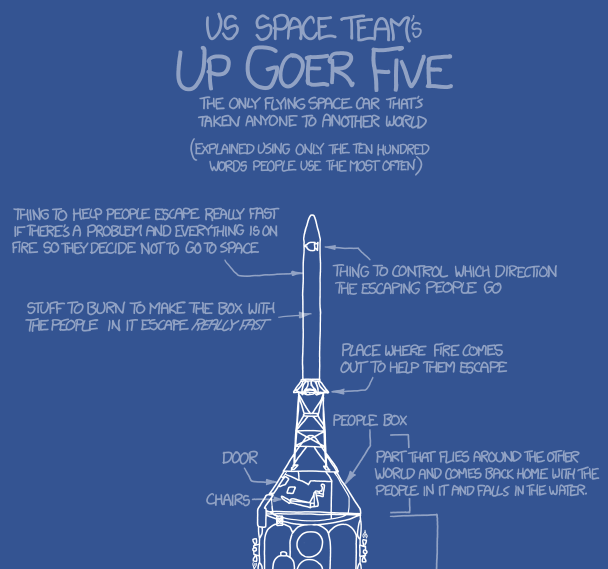
\includegraphics[width=\textwidth]{Slides/Design/Daten/up_goer_five_part.png}
	\end{figure}
	
	\column{0.5\textwidth}
	\begin{itemize}
		\item angemessene Leseschwierigkeit
		\begin{itemize}
			\item Satzlänge
			\item Wortlänge
			\item Vokabular
				%jargon, acronyme, worthäufigkeitslisten
		\end{itemize}
	\end{itemize}
\end{columns}
}


	
	


\section*{}
 \frame{\frametitle{}
 	\begin{center}
    		\huge Ende\\
    			Vielen Dank
	\end{center}
 	
 }
	
%Zahl der Betroffenen
	%weltweit
	%deutschland
	%vergleich zu anderen behinderungen

%Pers"onliche auswirkungen

%Was ist Analphabetismus?
	%analphabeten sind nicht dumm!
	%abstufungen von Analphabetismus
	%ursachen von analphabetismus

%Teilgruppen der Analphabeten
	%Legasteniker
	%lern schwache, lern behinderte
	%funktionale Analphabeten

%Demonstration wie sich analphabetismus anf"uhlt
	%Text oder Programm in fremder Sprache
		%Merkaartor in Niederl"andisch?

%Beeintr"achtigungen
	%lesen
	%errinerungsvermögen
	%"Denken "ubers Denken"
	%Orientierung (in dokumenten) und suche

%Design l"osungen
	%alphabetisierung.de
		%readspeaker.com
	%interactive visualization for low literacy users
		%nicht f"ur legastheniker
	%Textvermeidung
		% Zahlen werden von den meisten jedoch dennoch richtig identifiziert.

%Design testen
	%probanden finden
	%zusammenarbeit mit Probanden


\end{document}
